\documentclass{beamer}
\usetheme{Boadilla}

\usepackage[utf8]{inputenc}
\usepackage{amsmath, amssymb}

% colors
\usepackage{color}    
\usepackage[table]{xcolor}
\usepackage{themecolors}

% tikz stuff
\usepackage{tikz} 
\usetikzlibrary{positioning, shapes.multipart, arrows, arrows.meta, shadows, backgrounds, fit}

% isabelle blocks
\usepackage{listings}
\lstdefinelanguage{isabelle}{%
    keywords=[1]{type_synonym,datatype,fun,abbreviation,definition,proof,lemma,theorem,session,sessions,theories},
    keywordstyle=[1]\bfseries\color{isabelleouterblue},
    keywords=[2]{where,assumes,shows,and},
    keywordstyle=[2]\bfseries\color{isabelleoutergreen},
    keywords=[3]{if,then,else,case,of,SOME,let,in,O},
    keywordstyle=[3]\color{isabelleinnerblue},
    keywords=[4]{apply, by, done},
    keywordstyle=[4]\color{isabelleoutersalmon},
    morestring=[b]",
    stringstyle=\color{isabellequote},
    showstringspaces=false,
}
\lstset{%
  language=isabelle,
  escapeinside={&}{&},
  columns=fixed,
  extendedchars,
  basewidth={0.5em,0.45em},
  basicstyle=\ttfamily,
  mathescape,
}

\title{Stacking Correspondence}
\subtitle{Formal Verification of the Network Stack}
\author{Daniel Neshyba-Rowe}
\institute{Lewis \& Clark College}
\date{April 17, 2025}
\begin{document}
\begin{frame}
\titlepage
\end{frame}

% \begin{frame}
% \frametitle{Outline}
% \tableofcontents
% \end{frame}

\section{Introduction}

\subsection{The Network Stack}
\begin{frame}{The Network Stack}
    

    \begin{itemize}
        \item<1-> ``The network stack is an implementation of a computer networking protocol suite or protocol family.'' (wikipedia)
        \begin{itemize}
            \item<2-> Not a very helpful description
        \end{itemize}
        
    \end{itemize}
    

    \onslide<1,2>{
    \begin{figure}
        \centering
        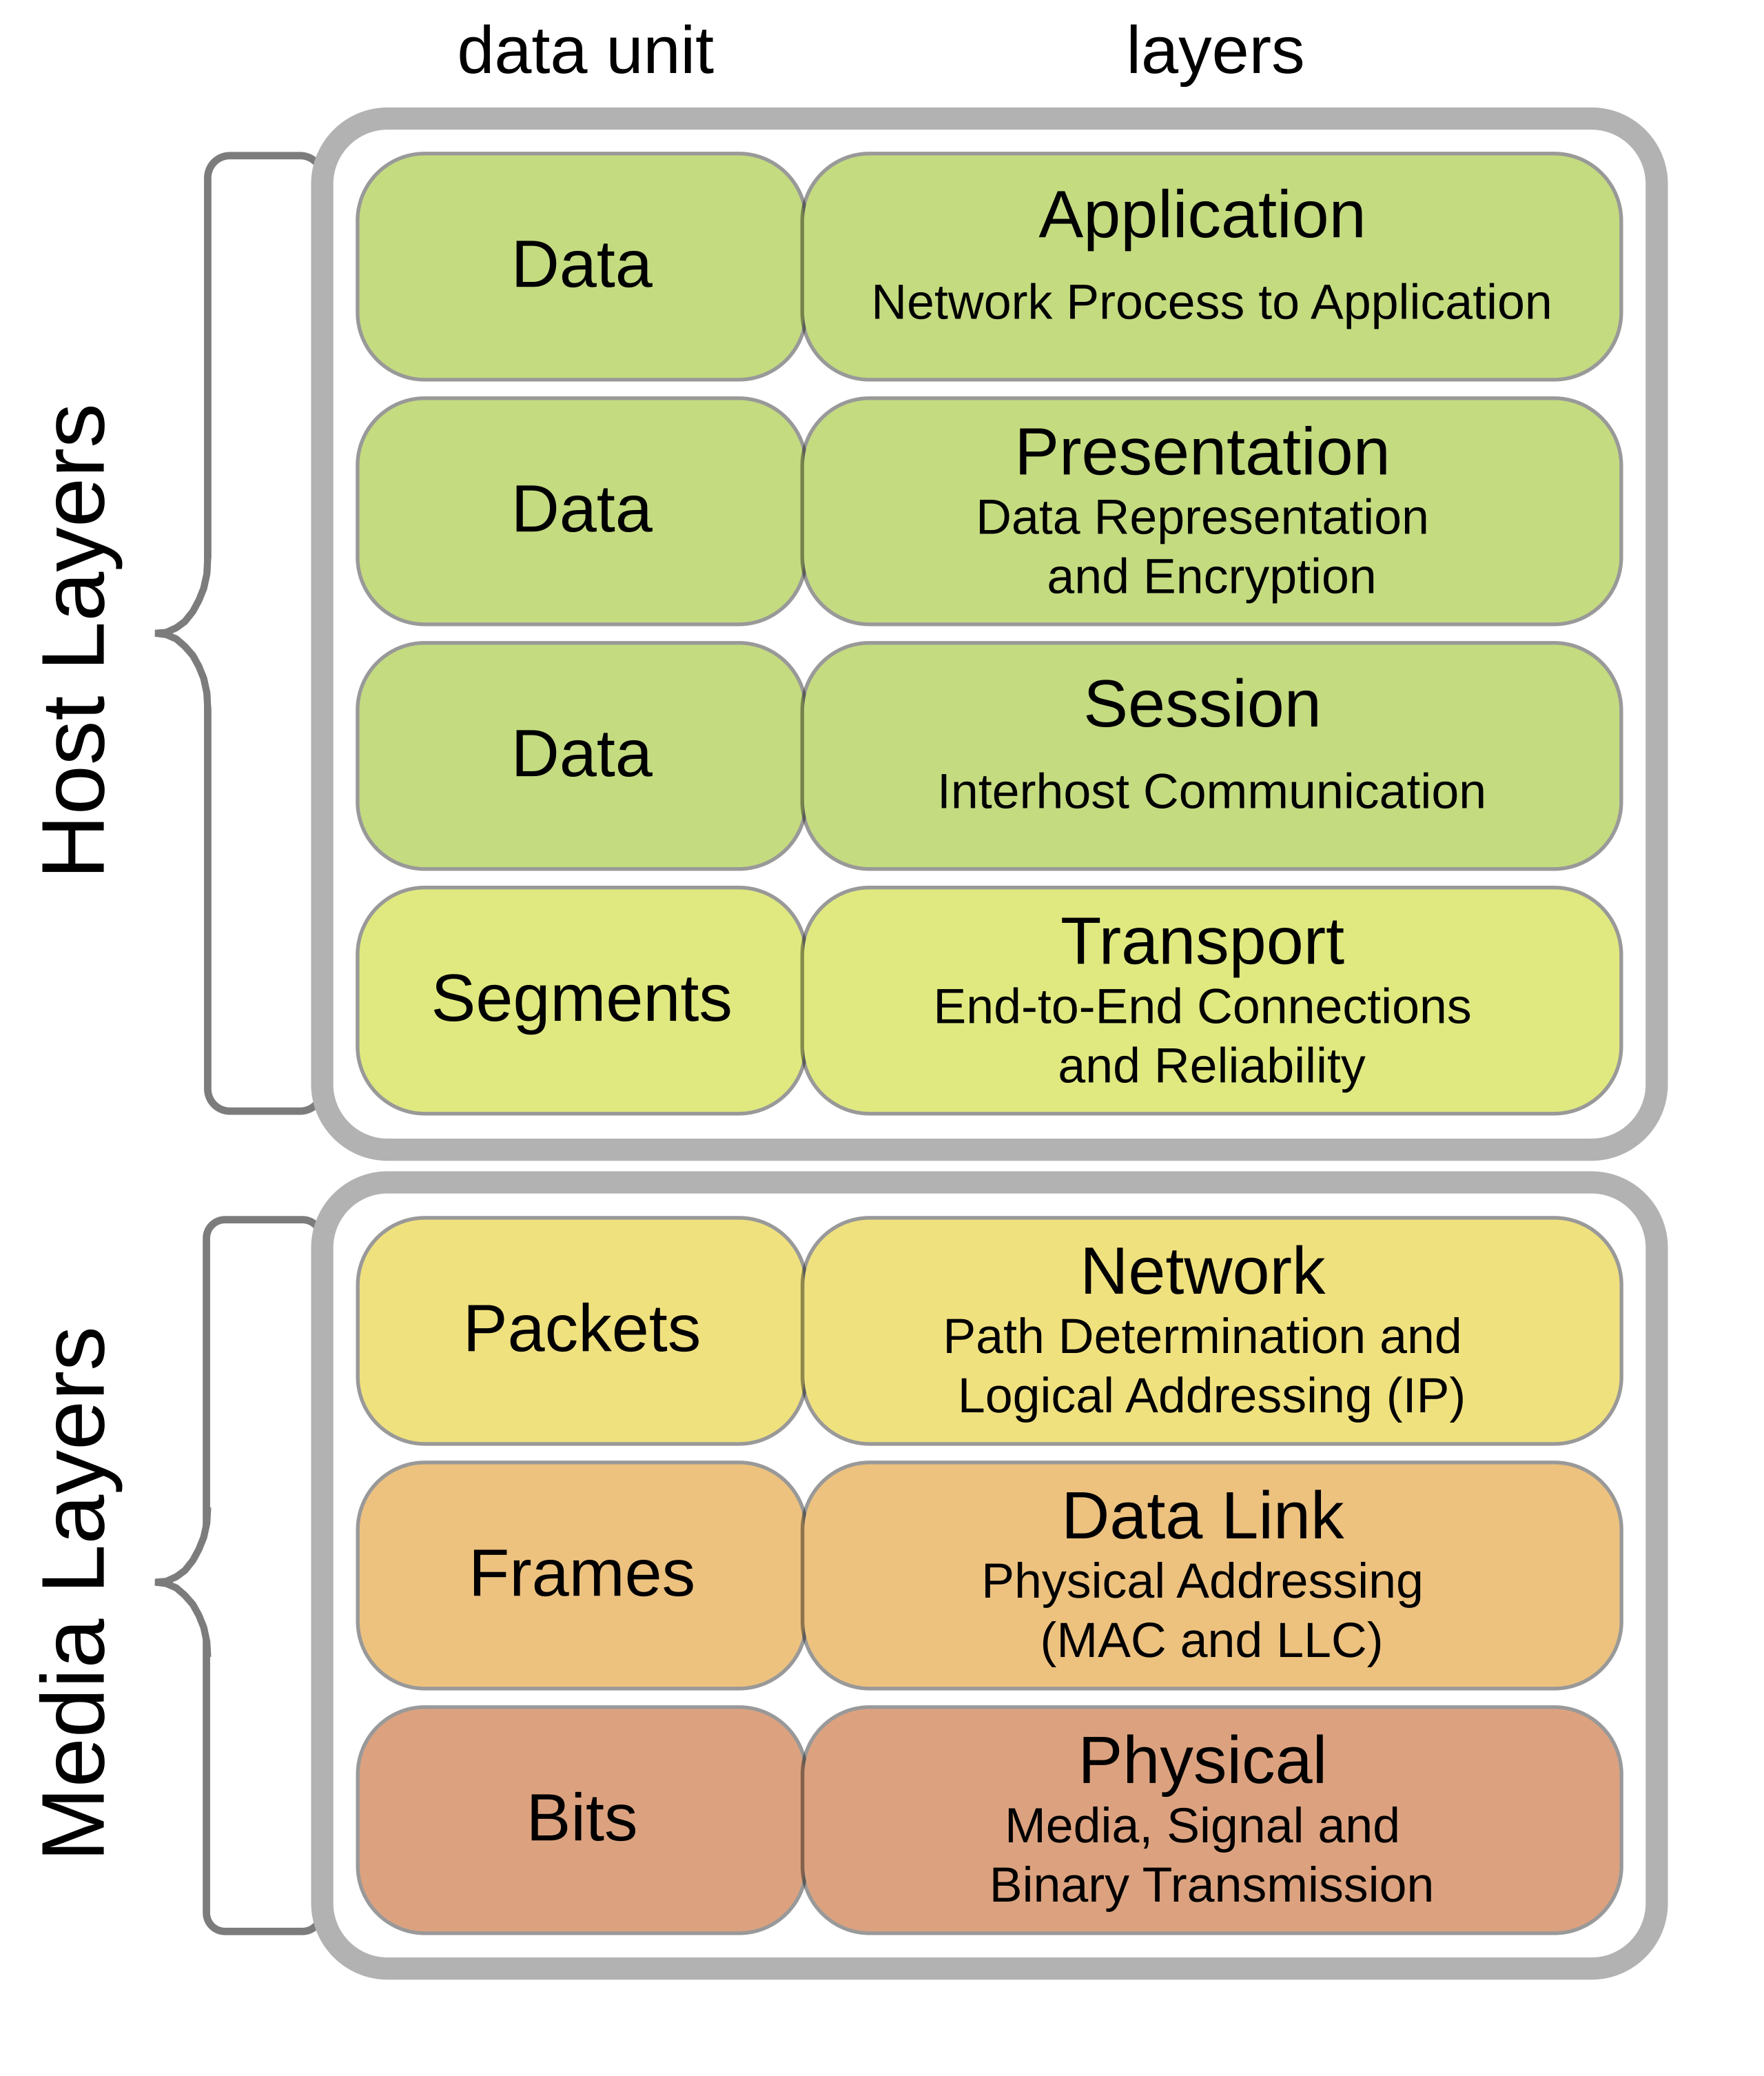
\includegraphics[width=0.4\linewidth]{../thesis_presentation/figs/wikipedia_OSI_Model_v1.svg.png}
        \caption{The OSI model, taken from Wikipedia}
        \label{fig:enter-label}
    \end{figure}
    }
\end{frame}

\begin{frame}{The Network Stack---Post Office analogy}
TODO: insert images here
\end{frame}

\begin{frame}{Verification}
Verification is proving ``it has no bugs.''
But what does that look like?
\vspace{20pt}\\

    \begin{columns}[t]
        \column{0.5\textwidth}
        \begin{itemize}
            \item imagine an ideal post office
            \item show that the ideal post office works great
            \begin{itemize}
                \item letters I send to you, you receive as written
            \end{itemize}
            \item look at a real post office
            \item show that the real post office works the same as the theoretical one
        \end{itemize}
        
        \column{0.5\textwidth}
        \begin{itemize}
            \item create an {\it abstract specification}
            \item show various {\it invariants} hold in the abstract specification 
            \vspace{1.65\baselineskip}\\
            \item create a {\it concrete specification}
            \item show the concrete specification {\it refines} the abstract specification
            \vspace{\baselineskip}\\
        \end{itemize}
    \end{columns}
    
\end{frame}

\begin{frame}<1,2>[label=ver_dif_tests]{Formal Verification is different from tests}
    In formal verification, we need rigorous mathematical proofs.
    
    Furthermore, these proofs should be verified
    by a \alert<2,3,4>{\it proof engine}.
    \vspace{20pt}\\
    
    One challenge with \alert<4>{system software} is that things
    frequently have a low chance of failing, but could still fail (e.g. two processes trying to access
    the same data at the same time---unlikely, but
    if handled poorly disastrous).
\end{frame}

\begin{frame}{Proof engines make proofs more rigorous}
    Infamously, people make misatkes.
    This is a big problem when formality is required.

    % TODO: split up into own slide? Ignore?
    Some examples of human error in proofs:
    \begin{itemize}
        \item Fifth Postulate
        \item All horses are the same color
    \end{itemize}

    What's the solution?
    Use software to automate checking proofs (a proof engine).

\end{frame}

\begin{frame}[fragile]{Isabelle --- the proof engine we use}
    Isabelle is one such proof engine.
    Isabelle is itself verified correct, and provides tools to prove mathematical statements.
    \begin{lstlisting}
lemma "2 + 2 = 4" by simp
    \end{lstlisting}
\end{frame}

\againframe<3,4>{ver_dif_tests}

\begin{frame}{System software is hard to verify}
    % TODO: decide: "embeded system" vs "system"
    System software is in charge of low-level operations.
    \begin{itemize}
        \item needs to be fast
        \item directly deals with memory and other hardware resources
    \end{itemize}
    These make verification tricky.
    So tricky, people thought it was impossible for a long time.
    \begin{itemize}
        \item until about 2009, most verification dealt with high-level abstract data structures and algorithms
        \begin{itemize}
            \item stacks, heaps, trees
            \item easily formalizable
            \item have to simply assume without proof that basic structures work as intended
        \end{itemize}
        \item in 2009, seL4 proved things from the ground up, only assuming hardware works correctly.
        \item but seL4 doesn't do anything on its own---it's a \textit{microkernel}.
    \end{itemize}
\end{frame}

\begin{frame}{seL4 as a microkernel}
    The job of a microkernel is to securely share resources
    (e.g. time, memory, access to network wires)
    between different processes
\begin{figure}[htpb]
    \centering
    \scalebox{0.5}{
    \begin{tikzpicture}[node distance=4cm]
        % styles
        \tikzstyle{cell} = [rectangle, minimum width=4.6cm, minimum height=3cm, text centered, draw=black]
        \tikzstyle{arrow} = [line width=2pt,->,>=latex,draw=gray]
        \tikzstyle{box} = [draw, rectangle, align=center, minimum width=11cm, inner sep=3ex]

        % wrap
        \node (mem0) [cell, fill=blue!80] {shared memory region};
        \node (PD1) [cell, fill=cyan!80, below left=20pt of mem0] {Protection Domain};
        \node (PD2) [cell, fill=green!80, below right=20pt of mem0] {Protection Domain};
        \node (mem1) [cell, fill=cyan!80, below=60pt of PD1] {memory region}; 
        \node (mem2) [cell, fill=green!80, below=60pt of PD2] {memory region}; 
        % % layers
        % \node[box, label={left:\rotatebox{90}{Higher-level}}, fit = (app_wrap) (app_unwrap)] (1) {};
        % \node[box, label={left:\rotatebox{90}{Transport}}, fit = (udp_wrap) (udp_unwrap)] (1) {};
        % \node[box, label={left:\rotatebox{90}{Network}}, fit = (ip_wrap) (ip_unwrap)] (1) {};
        % \node[box, label={left:\rotatebox{90}{Data Link}}, fit = (ethernet_wrap) (ethernet_unwrap)] (1) {};
        % \node[box, label={left:\rotatebox{90}{Physical}}, fit = (hardware_wrap) (hardware_unwrap)] (1) {};
        \node [color=red] at (0, -150pt) {blocked access};
        \node [color=green!200] at (-115pt, -180pt) {good access};

        % flow of information
        \draw [arrow, <->] (PD1) -- (PD2) node[midway, above] {notification};
        \draw [arrow, draw=green] (PD1) -- (mem1);
        \draw [arrow, draw=green] (PD2) -- (mem2);
        \draw [arrow, draw=green] (PD1) -- (mem0);
        \draw [arrow, draw=green] (PD2) -- (mem0);
        \draw [arrow, draw=red!40, -{> Square[black]}] (PD1) -- (mem2);
        \draw [arrow, draw=red!40, -{> Square[black]}] (PD2) -- (mem1);
    \end{tikzpicture}}

    
    \caption{A depiction of some core components of the seL4 microkernel}
    \label{fig:network-stack}
\end{figure}
    
\end{frame}















\subsection{Goals}
\begin{frame}
    \frametitle{Project Overview}
    \begin{itemize}
        \item Explore formal code
            \begin{itemize}
                \item lots of existing high-level verification
                \item seL4 first verified microkernel
                \item how far up can we push it?
            \end{itemize}
        \item Build a significant program correctly
            \begin{itemize}
                \item embedded system
                \item IPv6 networked fish tank thermometer
                \item network communication definitely not trivial
            \end{itemize}
    \end{itemize}
\end{frame}

\begin{frame}
    \frametitle{Goals for this part of the project}
        \begin{itemize}
            \item provide a roadmap for how our proofs should work
            \item start on some of the simpler parts of proof
        \end{itemize}
\end{frame}


\subsection{Approach}
\begin{frame}
    \frametitle{Prior work}
    \begin{itemize}
        \item Follow along with seL4's methodology for proofs
        \item Use seL4's existing tools
        \item Use existing specifications (network stack has been built before)
    \end{itemize}
\end{frame}


\subsection{Background}

\section{Methods}
\subsection{seL4}
\begin{frame}
    \frametitle{What do we need to write functional code?}
    \begin{itemize}
        \item seL4 is hard to work with
            \begin{itemize}
                \item use sDDF
                \item use microkit
            \end{itemize}
    \end{itemize}
\end{frame}
\begin{frame}
    \frametitle{How does software look in seL4?}
    \begin{itemize}
        \item PDs
        \item memory regions
    \end{itemize}
\end{frame}


\subsection{Overview of architecture}
\begin{frame}
    \frametitle{The network stack}
\begin{figure}[htpb]
    \centering
    \scalebox{0.55}{
    \begin{tikzpicture}[node distance=4cm]
        % styles
        \tikzstyle{cell} = [rectangle, minimum width=4.6cm, minimum height=1cm, text centered, draw=black]
        \tikzstyle{arrow} = [line width=2pt,->,>=latex,draw=gray]
        \tikzstyle{box} = [draw, rectangle, align=center, minimum width=11cm, inner sep=3ex]

        % wrap
        \node (app_wrap) [cell, fill=application!80] {Application on Computer A};
        \node (udp_wrap) [cell, fill=udp!80, below=30pt of app_wrap] {UDP wrap};
        \node (ip_wrap) [cell, fill=ip!80, below=30pt of udp_wrap] {IP wrap};
        \node (ethernet_wrap) [cell, fill=ethernet!80, below=30pt of ip_wrap] {Ethernet wrap};
        \node (hardware_wrap) [cell, fill=hardware!80, below=30pt of ethernet_wrap] {Hardware};

        % unwrap
        \node (app_unwrap) [cell, fill=application!80, right=14pt of app_wrap] {Application on Computer B};
        \node (udp_unwrap) [cell, fill=udp!80, below=30pt of app_unwrap] {UDP unwrap};
        \node (ip_unwrap) [cell, fill=ip!80, below=30pt of udp_unwrap] {IP unwrap};
        \node (ethernet_unwrap) [cell, fill=ethernet!80, below=30pt of ip_unwrap] {Ethernet unwrap};
        \node (hardware_unwrap) [cell, fill=hardware!80, below=30pt of ethernet_unwrap] {Hardware};

        % layers
        \node[box, label={left:\rotatebox{90}{Higher-level}}, fit = (app_wrap) (app_unwrap)] (1) {};
        \node[box, label={left:\rotatebox{90}{Transport}}, fit = (udp_wrap) (udp_unwrap)] (1) {};
        \node[box, label={left:\rotatebox{90}{Network}}, fit = (ip_wrap) (ip_unwrap)] (1) {};
        \node[box, label={left:\rotatebox{90}{Data Link}}, fit = (ethernet_wrap) (ethernet_unwrap)] (1) {};
        \node[box, label={left:\rotatebox{90}{Physical}}, fit = (hardware_wrap) (hardware_unwrap)] (1) {};

        % flow of information
        \draw [arrow] (app_wrap) -- (udp_wrap);
        \draw [arrow] (udp_wrap) -- (ip_wrap);
        \draw [arrow] (ip_wrap) -- (ethernet_wrap);
        \draw [arrow] (ethernet_wrap) -- (hardware_wrap);
        \draw [arrow] (hardware_wrap) -- (hardware_unwrap);
        \draw [arrow] (hardware_unwrap) -- (ethernet_unwrap);
        \draw [arrow] (ethernet_unwrap) -- (ip_unwrap);
        \draw [arrow] (ip_unwrap) -- (udp_unwrap);
        \draw [arrow] (udp_unwrap) -- (app_unwrap);
    \end{tikzpicture}}

    
    \caption{A simplified OSI model, showing the wrap and unwrap components of each layer. Arrows show flow of data. Session, presentation, and application layers are combined into a single ``higher-level'' layer---these layers are unnecessary for our use case of a simple thermometer.}
    \label{fig:network-stack}
\end{figure}
\end{frame}

\subsection{Formalizing program execution}
\subsection{What does it mean to verify a program?}

\section{Results}
\subsection{Current state of proofs}

\section{Discussion}
\subsection{Remarks/Conclusion}
\subsection{Pure function vs pure state transformation vs hybrid}
\subsection{Prior work}




\begin{frame}[fragile]
\frametitle{SIMPL language}
\begin{lstlisting}[language=isabelle]
type_synonym 's bexp = "'s set"
type_synonym 's assn = "'s set"

datatype (dead 's, 'p, 'f) com =
    Skip
  | Basic "'s $\Rightarrow$ 's"
  | Spec "('s $\times$ 's) set"
  | Seq "('s ,'p, 'f) com" "('s,'p, 'f) com"
  | Cond "'s bexp" "('s,'p,'f) com"  "('s,'p,'f) com"
  | While "'s bexp" "('s,'p,'f) com"
  | Call "'p"
  | DynCom "'s $\Rightarrow$ ('s,'p,'f) com"
  | Guard "'f" "'s bexp" "('s,'p,'f) com"
  | Throw
  | Catch "('s,'p,'f) com" "('s,'p,'f) com"
\end{lstlisting}
\end{frame}


    
\end{document}

